\documentclass{article}

\usepackage{datetime}
\usepackage[utf8]{inputenc}

\usepackage{mathtools}
\usepackage{graphicx}
\usepackage{float}
%\usepackage{verbatim}
%\usepackage[margin=25mm]{geometry}
\setlength{\parskip}{\medskipamount}
\setlength{\parindent}{0pt}

\begin{document}

\title{Assignment 3 and 4}
\author{Emil Daijiro Grønnbeck \& Øystein Tandberg}
\date{\today}
\maketitle

\section{System overview}
The code is written in Scala and Java. To build this project we used a tool called Simple Build Tool (sbt) \cite{sbt}. As visualization for both the Flatland and the Tracker problem we wrote the outputs of the agens as JSON to a output-file and visualizated the steps in the browser with help of javascript. 

\begin{figure}[H]
  \centering
    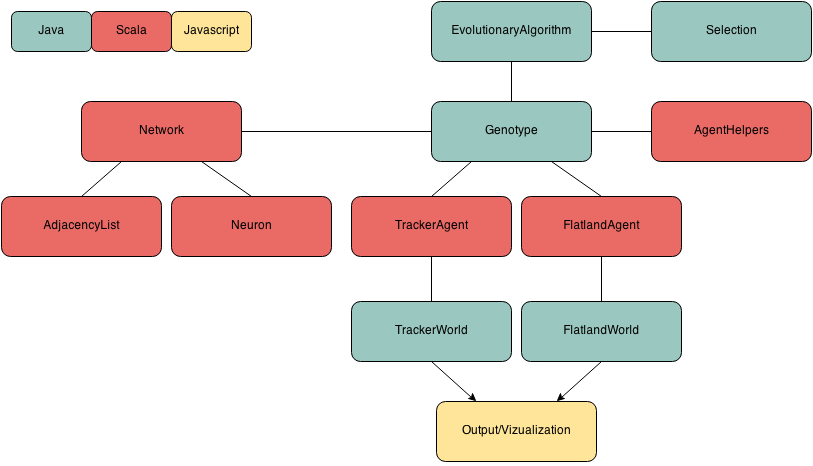
\includegraphics[width=1.0\textwidth]{img/class_diagram}
    \caption{Class hierarcy for both problems. Color labels is to the top-right of the figure. This makes it easy to add new problems to the codebase.}
\end{figure}

The program runs from the EvolutionaryAlgorithm class which wires up the EA and agents to run simulations on the given problem. 

\section{Evolving Neural Networks for a Flatland Agent}
\subsection{EA-parameters}
\begin{center}

\begin{tabular}{p{5cm} | r}
\textbf{Parameter} & \textbf{Value} \\
\hline
Population & 75 \\
Maximum iterations & 200 \\
Elitism & 5 \\
Tournament size & 10 \\
Tournament epsilon & 0.2 \\
Mutation percent & 0.05 \\
Crossover rate & 0.2 \\
\hline
\end{tabular}
\end{center}

To find these parameters we tried dozens of complete runs, also with different parent mate selection and adult selection mechanisms. In the end we ended up using \textbf{Tournament selection} along with \textbf{Generation Mixing} in the Evolutionary algorithm to evolve a fairly good agent to move around in the Flatland world.

\subsection{Fitness function}
\begin{tabular}{l l}
Food pickups & $\sim f$ \\
Poison pickups & $\sim p$ \\
\end{tabular}

$f(simulation) = f - p$

\subsection{ANN design}

\begin{figure}[H]
  \centering
    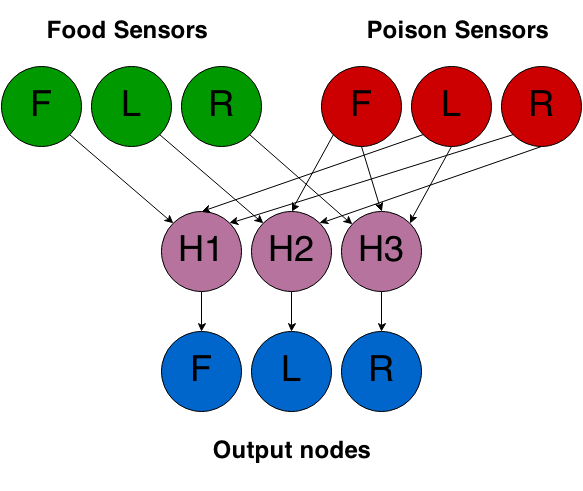
\includegraphics[width=0.5\textwidth]{img/Flatland_network}
    \caption{Artificial Neural Network for the Flatland Agent.}
\end{figure}

Three hidden nodes represents the layer between the input sensors and the output nodes. The main idea of the hidden nodes is to understand that the poison is negative and food is positive for the final outputs. The food input sensors is linked to the "same" hidden node, while the poison input sensors is linked to the "opposite" hidden node. 

The weights in this artificial neural network can have values $[-1, 1]$. Inside each neuron the Sigmoid function is used to calculate if the neuron is activated or not. The input to the Sigmoid function is the weight of each input node that is activated. The neuron will be activated if:

\begin{center}
	$\frac{1}{1 + \exp^{-x}} \geq 0.5$
\end{center}

Where x is the sum of weights times each connected neurons activation (0 or 1).

The weights is evolved from the evolutionary algorithm. The bitstring from the EA is splitted up in groups of 8 bits per weight and then converted into a number in the weight range. This is of course easy to change with parameters to have higher precision to the weights in the ANN, and we found out that 8 bits as one weight was a good number to produce good results. With $x$ bits to each weight, our network with 12 edges, the EA will have to deal with $12x$ bits.

\subsection{Static vs dynamic runs}
Hard coded runs vs $FPD(x, y)$ runs


\newpage
\section{Evolving Neural Networks for a Minimally-Cognitive Agent}
\subsection{System overview}
The class diagram of the system is described above, we used the same techniques to do the wiring from Agent to World as in the Flatland problem. The big difference in this problem was the network. \textcolor{red}{TODO: Write about the network implementation.}


The genotype retrieved from the EA was splitted up into \textcolor{red}{4?}groups in the step of converting it to a phoenotype. This 4 groups is the main weights, bias, gain and time thresholds. Like in the Flatland agent the bits is converted to a number between the maximum and minimum for each value.

\begin{center}
\dots101010110{\LARGE11101010}111100101\dots
\end{center}

As an example, the raised binaries above (which is part of the weight group of 22 weights) will convert of one weight that will have a value of 4.18.

\subsubsection{Parameters in the EA to evolve the CTRNN}
\begin{center}
\begin{tabular}{p{5cm} | r}
\textbf{Parameter} & \textbf{Value} \\
\hline
Population & 75 \\
Maximum iterations & 200 \\
Elitism & 5 \\
Tournament size & 10 \\
Tournament epsilon & 0.2 \\
Mutation percent & 0.05 \\
Crossover rate & 0.2 \\
\hline
\end{tabular}
\end{center}


\subsection{Parameteres to catch all objects}


\subsection{Significant modifications}
\subsubsection{Tracker scenario}
Feks height = 100

\subsubsection{CTRNN topology}
Bytte antall hidden nodes

\subsubsection{CTRNN variables}
Feks weights in $[-100, 100]$

\subsection{Weight analysis}
Dunno Dunno Dunno Dunno Dunno 


\begin{thebibliography}{9}
	\bibitem{sbt}
	  Simple Build Tool, http://www.scala-sbt.org/
\end{thebibliography}

\end{document}